\section{Datasets}
\label{sec:datasets}
For testing the bootstrapping loss function and curriculum learning as well as measuring the performance of the roaad detection system, two datasets have been used. Both datasets involve the task of semantic segmentation of images, more precisely the task of extracting roads from aerial images. The first dataset, Massachusetts Roads Dataset, is provided by \cite{MnihThesis} and have been used in other works. The second dataset, Norwegian Roads Dataset, has been created from publicly available sources specifically for this thesis. Differences, similarities and challenges of employing these datasets will be further discussed below.\\

\subsection{Massachusetts Roads Dataset}
The Massachusetts Roads Dataset contains aerial images depicting urban, suburban and rural areas in the state of Massachusetts, USA. In all, the dataset consists of 1171 aerial images, where each image is $1500\times 1500$ pixels in size. 1108 of these images have been randomly assigned to the training set. The remaining 49 and 14 images can be found in the test and validation set. The dataset covers an area of approximately 2600 square kilometers in total, which gives a \ac{GSD} of 1.0 meter per pixel.\\

Each aerial image have an accompanying identically sized binary label image which indicate whether a pixel in the aerial image belongs to either the road or non-road class. Road centerline vectors retrieved from the OpenStreetMap project were used to generate the labels images. The vectors were rasterized as white lines with a line thickness of 7 pixels \citep{MnihThesis}, which based on the \ac{GSD} is equivalent to 7 meters on the ground. An aerial image and label image pair from this dataset can be seen in Figure \ref{fig:mass_roads_example}.\\

\begin{figure}
\begin{subfigure}{0.48\textwidth}
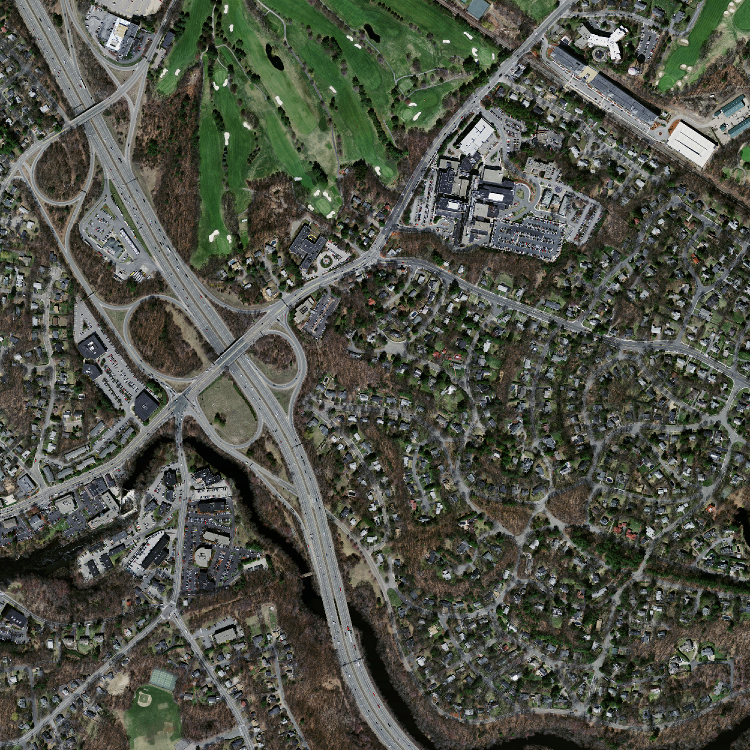
\includegraphics[width=\linewidth]{figs/datasets/Mass_roads_data_example2.png}
\caption{Aerial image} \label{fig:mass_roads_example_data}
\end{subfigure}
\hspace*{\fill} % separation between the subfigures
\begin{subfigure}{0.48\textwidth}
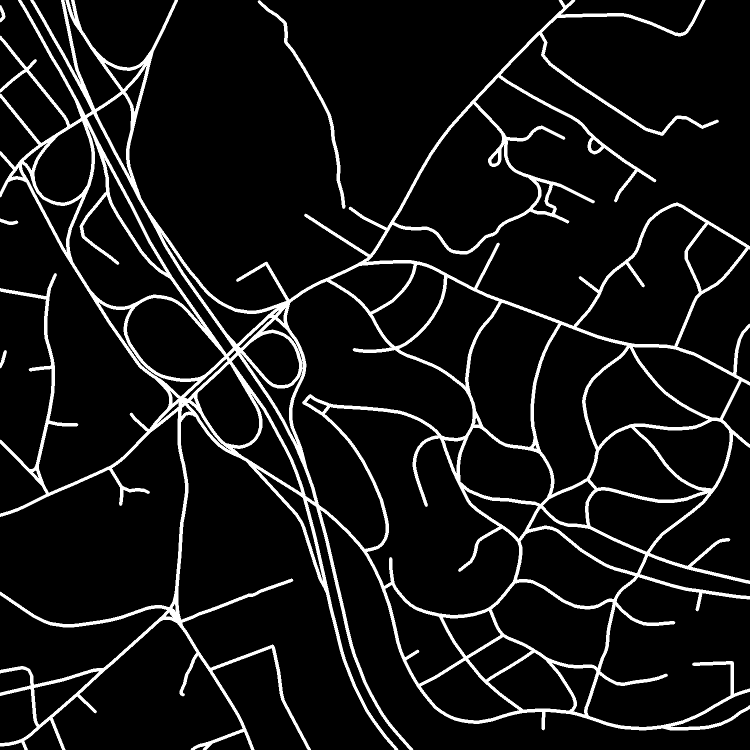
\includegraphics[width=\linewidth]{figs/datasets/Mass_roads_label_example2.png}
\caption{Label image} \label{fig:mass_roads_example_label}
\end{subfigure}
\hspace*{\fill} % separation between the subfigures
\caption{Image and label example taken from test set in Massachusetts Roads Dataset.} \label{fig:mass_roads_example}
\end{figure}


There are many reasons for using this dataset for conducting experiments related to the research questions.  The task involves semantic segmentation of roads based exclusively on aerial color images which is arguable a hard task, and might justify the use of a large model for training, such as a \ac{CNN}. The dataset has also been used in other works, which enables comparisons between the results obtained in this thesis and results obtained in other works. Additionally, the labels have been generated from existing map data, and therefore contains many instances of naturally occurring inconsistent labelling. This is compelling in relation to the research questions of this thesis.\\

Aerial image datasets typically suffer from two distinct types of label noise, which \cite{Mnih_aerial_images_noisy} have named omission and registration noise. The dataset is generated from existing map data, which has some deficiencies when coupled with supervised learning. There are many instances of omission noise in this dataset, where smaller roads and parking areas have not been marked as road class pixels in the label images. These omissions are most likely perfectly acceptable for map purposes, but might negatively impact the performance of a classifier.  Because unlabelled paved areas share a high spectral similarity to roads, this type of inconsistent labelling might compel the model to minimize the loss by learning complicated distinctions between surfaces that are essentially the same thing \todo{Show examples}.\\

There are also instances of registration noise in this dataset. this happens when the roads have been marked in the label image, but there are a misalignment between the road found the the aerial image and the road centerline vector from the map data. Additionally, the road centerline vectors have in many cases been rasterized with the incorrect line thickness, which might cover to much or not enough depending on the road's lane width. The result is a lot of aerial image pixels have been assigned the wrong class, and might impact the learning negatively. Just like omission noise, slightly misaligned road centerline vectors does probably not matter too much for map purposes, whereas they create a lot of inconsistent examples in a machine learning dataset.


%\subsection{Massachusetts Roads Dataset}

\subsection{Norwegian Roads Dataset}
In addition to the Massachusetts Roads Dataset \citep{MnihThesis}, the proposed methods have been tested with the Norwegian Roads Dataset. This dataset was constructed from aerial images retrieved from Kartverket, which depicts both rural, suburban and urban areas from different locations in Norway. The entire dataset consists of 1225 aerial images, each being $1536\times 1536$ pixels in size. 1100 of them have been randomly assigned to the training set, 75 the test set, and the remaining images were put in the validation set. Even though there are more aerial images in this dataset compared to the Massachusetts Roads Dataset, it only covers an area of around 1910 square kilometers. This is because of a much lower \ac{GSD} of about 0.66 meters per pixel. \\


The label images for this dataset have been generated from road centerline vectors found in the publicly available topographic vector database, N50, provided by \cite{Kartverket}. Unlike the Massachusetts Roads Dataset, the centerline vectors have been rasterized with a variable line thickness. This is possible because all road segment in N50 have a set of properties, which can be utilized for determining a custom line thickness. The actual thickness for each road type have been based on numbers found in a road specification manual published by the Norwegian Public Roads Administration \citep{Norwegian_road_manual}. The road segment properties and line thickness for each road type are listed in Table \ref{tab:road_rules}. Roads which are underground and can not be seen from aerial imagery, have also been removed from the rasterized label images.\\

The aerial images have been taken from over 30 different locations in Norway, and offers a large variety of topographical features. There are images depicting coastline, rivers, mountain terrain, snow, cultivated land and forests. Compared to Massachusetts Roads Dataset the aerial images of this dataset have been sampled from a much larger areas. \\

Furthermore, the aerial images might present a challenge in terms of image quality. Some of the images have a lower quality, and vary in terms of color balance, and contrast. There are also aerial images which have been stitched together from images captured by aerial surveys conducted at occasions.\\

The quality of the the generated label maps might also present a challenge to a machine learning algorithm. There are both omission and registration errors present in many of the label images. Compared to Massachusetts Roads Dataset there are a much higher degree of registration errors. The road centerlines in N50 generally appear more coarse, and result in less overlap between roads in the aerial image and the raster lines in the label image. This is especially evident in road centerline vectors for divided highways. Instead of having centerline vectors for both roadways, there are only one placed between the roadways on the median. Visual examples of missing and misplaced labels can be seen in Figure \ref{fig:norwegian_roads_examples_n50}.\\

\begin{figure}[h]
\begin{subfigure}{0.31\textwidth}
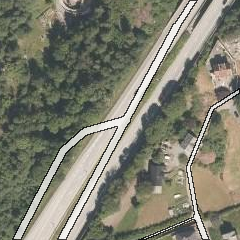
\includegraphics[width=\linewidth]{figs/datasets/nor_examples/1191_highway_n50.png}
\caption{Divided highways} \label{fig:norwegian_roads_highway_n50}
\end{subfigure}
\hspace*{\fill} % separation between the subfigures
\begin{subfigure}{0.31\textwidth}
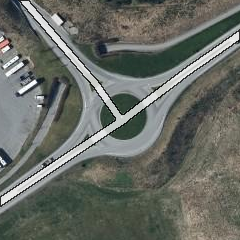
\includegraphics[width=\linewidth]{figs/datasets/nor_examples/1177_roundabout_n50.png}
\caption{Roundabout} \label{fig:norwegian_roads_roundabout_n50}
\end{subfigure}
\hspace*{\fill} % separation between the subfigures
\begin{subfigure}{0.31\textwidth}
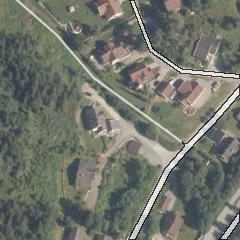
\includegraphics[width=\linewidth]{figs/datasets/nor_examples/1157_missing_n50.png}
\caption{Private road} \label{fig:norwegian_roads_missing_n50}
\end{subfigure}
\hspace*{\fill} % separation between the subfigures
\caption{Examples of inconsistent labelling found in the Norwegian Roads Dataset N50.} \label{fig:norwegian_roads_examples_n50}
\end{figure}

In addition to the set of label images generated from N50, the dataset also include an alternate set of label images generated from the road centerline vector database, Vbase \citep{Kartverket_vbase}, which have more accurate road centerline vectors. There are still omission and registration errors present in this label image set, but to a less extent. Surfaces that share spectral similarities to asphalt, such as private roads and parking areas have not been marked, similar to the Massachusetts Roads Dataset. The difference in accuracy between N50 and Vbase, can be seen by comparing Figure \ref{fig:norwegian_roads_examples_n50} and Figure \ref{fig:norwegian_roads_examples_vbase}. A minor downside of using this alternate vector database is that Vbase provide fewer road segment properties, which have resulted in smaller of set of line thicknesses applied to the label images.\\

\begin{figure}[h]
\begin{subfigure}{0.31\textwidth}
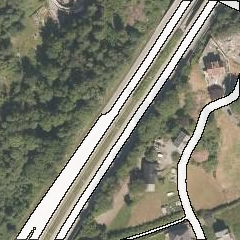
\includegraphics[width=\linewidth]{figs/datasets/nor_examples/1191_highway_vbase.png}
\caption{Divided highways} \label{fig:norwegian_roads_highway_vbase}
\end{subfigure}
\hspace*{\fill} % separation between the subfigures
\begin{subfigure}{0.31\textwidth}
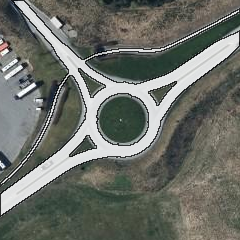
\includegraphics[width=\linewidth]{figs/datasets/nor_examples/1177_roundabout_vbase.png}
\caption{Roundabout} \label{fig:norwegian_roads_roundabout_vbase}
\end{subfigure}
\hspace*{\fill} % separation between the subfigures
\begin{subfigure}{0.31\textwidth}
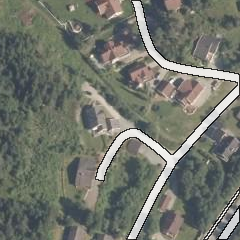
\includegraphics[width=\linewidth]{figs/datasets/nor_examples/1157_missing_vbase.png}
\caption{Private road} \label{fig:norwegian_roads_missing_vbase}
\end{subfigure}
\hspace*{\fill} % separation between the subfigures
\caption{Examples of road centerline vector quality in Vbase.} \label{fig:norwegian_roads_examples_vbase}
\end{figure}

\begin{table}[htp]
\caption{Raster line thickness and road segment filtering rule for each type of road. A margin of 10\% is removed from the line thicknesses, which are based on numbers found in the road specification manual.}
\begin{center}
\begin{adjustbox}{max width=\textwidth}
\begin{tabular}{+l ^l ^r}\hline
		 \rowstyle{\bfseries}
 		 Road type & Road segment property & Line thickness\\\hline
 		 Dirt road & OBJTYPE=Traktorveg & 2.50 m\\
 		 Trail & OBJTYPE=Sti & 1.50 m\\
 		 pedestrian road & OBJTYPE=GangSykkelveg & 2.25 m\\
 		 Highway & MOTORVEGTYPE=motorveg & 10.80 m\\
 		 International E-road network & VEGKATEGORI=E & 6.30 m\\
 		 Norwegian national road & VEGKATEGORI=R & 5.85 m\\
 		 municipal road & VEGKATEGORI=K & 4.95 m\\
 		 Private road & VEGKATEGORI=P & 3.50 m\\\hline
\end{tabular}
\end{adjustbox}
\end{center}
\label{tab:road_rules}
\end{table}

The dataset were constructed by using QGIS, an open source geographic information system application. The application enables viewing and editing of map data, but also provides a Python interface. A script to create label images was developed, which takes the map coordinates associated with each corner of an aerial image, and generates a raster image of road centerline vectors found inside that area. The resulting raster images can be used as target maps in supervised learning. \\

\begin{figure}
\begin{subfigure}{0.32\textwidth}
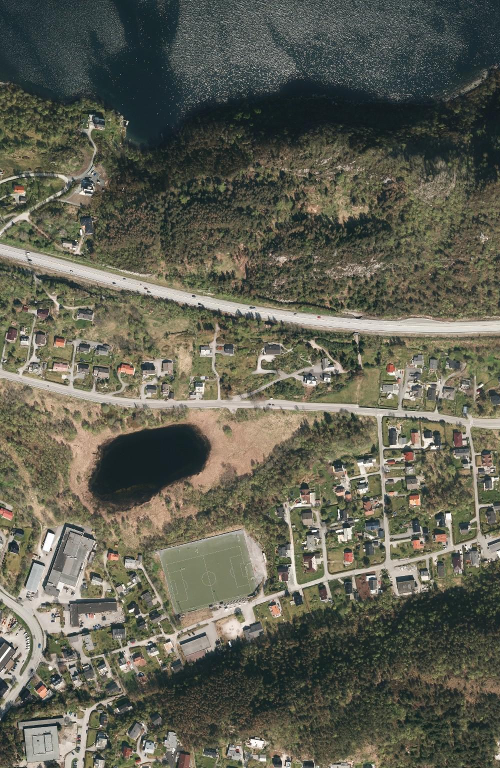
\includegraphics[width=\linewidth]{figs/datasets/Norwegian_roads_data_example2.png}
\caption{Aerial image} \label{fig:norwegian_roads_example_data}
\end{subfigure}
\hspace*{\fill} % separation between the subfigures
\begin{subfigure}{0.32\textwidth}
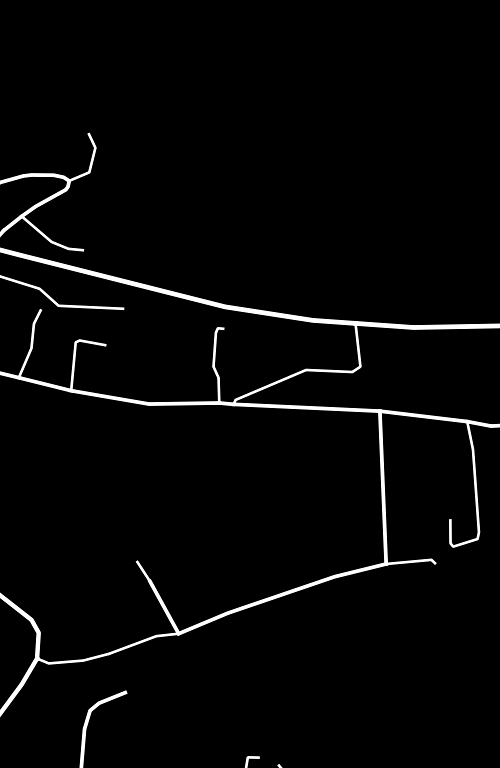
\includegraphics[width=\linewidth]{figs/datasets/Norwegian_roads_label_example2.png}
\caption{Label image} \label{fig:norwegian_roads_example_label}
\end{subfigure}
\hspace*{\fill} % separation between the subfigures
\begin{subfigure}{0.32\textwidth}
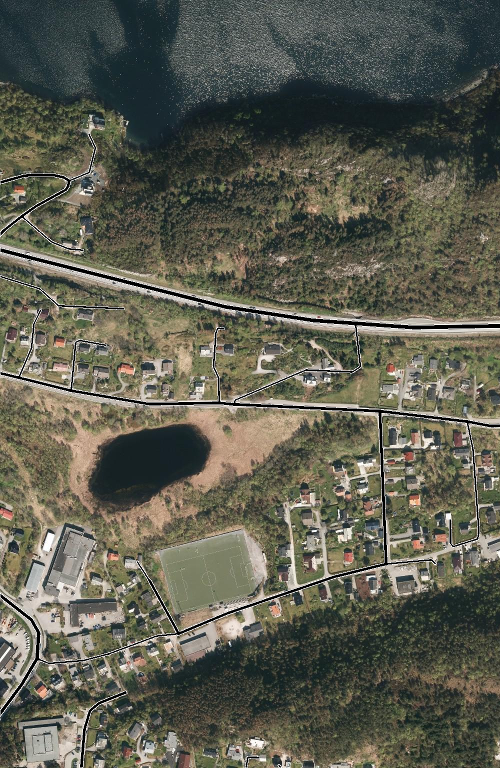
\includegraphics[width=\linewidth]{figs/datasets/Norwegian_roads_overlay_example2.png}
\caption{Overlay image} \label{fig:norwegian_roads_example_overlay}
\end{subfigure}
\hspace*{\fill} % separation between the subfigures
\caption{Example taken from test set in Norwegian Roads Dataset N50.} \label{fig:norwegian_roads_example}
\end{figure}

An aerial image and it's corresponding label image from the Norwegian Roads Dataset N50 can be seen in Figure \ref{fig:norwegian_roads_example}, and Figure \ref{fig:norwegian_roads_example_overlay} shows the same label image superimposed on the aerial image. Observe that some roads are missing from the label image, as well as the ground truth not covering the roads properly. \\
